%!TEX encoding = UTF-8 Unicode
%!TEX program = xelatex

\documentclass[bachelor]{ustcthesis}
% bachelor|master|doctor
\usepackage{ustcextra}
\graphicspath{{figures/}}
\bibliographystyle{ustcauthoryear}
% \bibliographystyle{ustcnumerical}

\renewpagestyle{front}[\zihao{-5}]{
    \sethead{}{应用商店系统概要设计}{}
    \setfoot{}{\thepage}{}
    \headrule
}
\renewpagestyle{main}[\zihao{-5}]{
    \sethead{}{应用商店系统概要设计}{}
    \setfoot{}{\thepage}{}
    \headrule
}
\newcommand{\HRule}{\rule{\linewidth}{0.5mm}}
\newcommand{\tabincell}[2]{\begin{tabular}{@{}#1@{}}#2\end{tabular}}

\begin{document}



\begin{titlepage}
\begin{center}
~\\[5cm]
\HRule \\[0.4cm]
{\huge \bfseries 应用商店系统\\概要设计}\\[0.4cm]
\HRule \\[1.5cm]

\begin{tabular}{ccc}
  & 人员 & 日期 \\ 
拟制 & 董恒\ 李楠\ & 2019-5-9 \\ 
评审人 & 董恒\ 李楠\ & 2019-5-10 \\ 
批准 & 董恒\ 李楠\ & 2019-5-11 \\ 
签发 & 董恒\ 李楠\ & 2019-5-12 \\ 
\end{tabular} 

\end{center}
\end{titlepage}



\frontmatter
\begin{abstract}
    本说明是软件工程-应用商店系统案例研究项目软件产品的总体设计和实现说明,记
    录了系统整体实现上技术层面上的考虑,并且以需求说明作为依据,同时该文档将作为产品
    实现、特性要求和控制的依据。


    本阶段已在系统的需求分析研究的基础上,对应用商店系统做概要设计。该阶段正式进
入了实际开发阶段,它的目的就是进一步细化软件设计阶段得出的软件总体概貌,把它加工成
在程序细节上非常接近于源程序的软件表示。概要设计说明书主要解决了实现本系统需求的程
序模块设计问题。
\keywords{软件工程\zhspace{}应用商店系统 \zhspace{} 概要设计}

\begin{table}[htbp]
\centering
\caption{缩略词清单} \label{tab:abbr}
\begin{tabular}{|c|c|c|}
    \hline
    缩略语 & 英文全名 & 中文解释 \\
    \hline
    app & application & 应用\\
    \hline
    dev & developer & 开发者 \\
    \hline
    inter & interface & 接口 \\
    \hline
    info & information & 信息 \\
    \hline
    passwd & password & 密码 \\
    \hline
\end{tabular}
\end{table}
    

\end{abstract}

\tableofcontents
\listoffigures
\listoftables
% \listofalgorithms  % 算法索引,如不需要,可直接注释掉本行
% \begin{notation}

%\centering
%XX 软件需求规格说明书

%关键词:能够体现文档描述内容主要方面的词汇。
 
%摘要:


\centering
\begin{tabular}{rl}
$\ln x$ & natural logarithm $\log_ex$ \\
$\log x$ & common logarithm $\log_{10}x$ \\
$x\ \mathrm{mod}\ y$ & remainder \\
\end{tabular}

\end{notation}


\mainmatter
\section{工具简介}
\label{sec:intro}
``违反编码规范的缺陷检测工具''(以下简称本工具)是根据NASAC2018软件原型命题竞赛组 
2018年10月21日晚发布的竞赛题目,
由中国科学技术大学计算机科学与技术学院张昱老师于10月22日
联络2018级硕士研究生张宇翔组队研制。
本参赛队由队长张宇翔、2016级本科生邓胜亮(10月23日加入)、
2018级硕士研究生李森(10月26日加入)组成,
工具研发的起止时间为2018年10月22日至11月10日;
张昱老师进行全程指导。

本参赛队利用 \href{https://clang.llvm.org/}{Clang 7.0.0} 
提供的工具框架
设计实现了具有可配置、易扩展的自动化违反编码规范的缺陷检测工具。
该工具提供函数参数合法性检查、函数错误返回码处理检查、
变量按需初始化检查、头文件自包含检查、循环依赖检查、
函数头注释检查、标识符命名检查等,
产生的诊断信息内容全面、可读性强。
用户可以方便地配置工具的行为,扩展其功能。

\subsection{功能简介}
\label{sec:intro:func}
该工具能够进行的检查如下:

\begin{itemize}
\item {\bf 函数参数合法性检查}
检查代码中模块对外接口是否进行了合法性检查。

\item{\bf 函数错误返回码处理检查}
检查在调用提供了错误指示机制的函数后,是否立即检查了错误指示。

\item{\bf 变量按需初始化检查}
检查代码中是否存在冗余的初始化。

\item{\bf 头文件自包含及循环包含检查}
检查头文件是否自包含且没有循环依赖。

\item{\bf 函数头注释检查}
检查函数头注释风格是否一致、注释中是否只有格式没有内容、是否说明了必要的信息、未注释的函数是否需要补充注释。

\item{\bf 标识符命名检查}
指出函数、变量名中的非英文单词,并对英文变量名提供常见的缩写建议。
\end{itemize}

所有检查的结果在汇报时都会指出其在源码中对应的位置(包括文件路径、行号、列号),方便用户进行修改。
各功能具体的实现细节将在 \S\ref{sec:core} 进行介绍。

\subsection{使用说明简介}
\label{sec:intro:usage}

该工具为命令行工具,用户通过提供命令行参数,对工具进行以下配置:

\begin{itemize}
    \item 关闭指定的一个或多个检查;
    \item 指定英文词典、缩写词典的位置;
    \item 指定返回错误码的函数列表的位置;
    \item 指定要检查的项目的编译命令列表位置;
    \item 指定要检查的文件或目录;
\end{itemize}

除了提供命令行选项以外,用户可以自行删减、扩充英文词典、缩写词典、返回错误码的函数列表,
从而方便地根据实际需要来定制工具的行为。

关于以上配置方式的具体说明见 \S\ref{sec:usage} 一节。

\chapter{总体概述}

本节描述影响产品和产品需求的一般因素。由以下4个部分构成。 有一点需说明的是本节不描述具体的需求,只是使那些将要描述的具体需求更易于理解。
\section{软件概述}
\subsection{项目介绍}
应用商店的开发与时俱进,现在出现的PC端与手机端应用商店出现了严重的割裂,
而且应用的质量得不到保证、用户的反馈得不到及时的回应、开发者的合理权益得不到保障、
用户需要专门花时间去找应用等等问题层出不穷。

现在出现的应用商店无法解决这样问题,这也是本项目出现的主要原因,
即构建一个面向未来的、可拓展的、友好的应用商店系统。
以达到全面替代当前的各种应用商店的目的。


\subsection{产品环境介绍}

本项目构成一个独立的体系而且完全自我包含。

\section{软件功能}
为了便于设计和理解,将软件的功能分为三个组块,即开发者端、服务器端、用户端。


下面详细介绍。

\subsection{开发者端}
针对开发者,我们需要设定开发者是普通的应用程序开发人员甚至是非专业的,为了激发开发的参与,
本系统需要简化应用开发的门槛,因而开发者端需要尽可能简化。
\begin{itemize}
\item 应用管理

	\begin{itemize}
	\item 应⽤上传
	\item 应用更新
	\item 应用删除
	\end{itemize}
\item 信息反馈
	\begin{itemize}
	\item
	应⽤信息查询与管理
	\begin{itemize}
		\item 下载量
		\item 评论
		\item 回复
	\end{itemize}
	\item 收⼊查询与管理
	\begin{itemize}
		\item 提现
		\item 转账
	\end{itemize}
	\end{itemize}

\item \color{red}{应用开发}
	\begin{itemize}
		\item \color{red}{代码编辑}
		\item \color{red}{代码编译与运行}
		\item \color{red}{debug功能}
	\end{itemize}
\end{itemize}
	

\subsection{服务器端}
服务器端是一个增加了某些特殊功能的数据库,需要存储开发者、应用、用户的信息,以及相关的触发操作,
下面的列表详细地说明了其功能。

\begin{itemize}
\item 开发者管理系统
	\begin{itemize}
	\item 开发者信息维护
		\begin{itemize}
		\item 注册与注销
		\item 个人基本信息
		\item 开发的应用
		\end{itemize}
	\item 反馈内容
		\begin{itemize}
			\item 收入查询
			\item 收入提现
			\item 应用评分与评论
		\end{itemize}
	\end{itemize}
\item 应用管理系统
	\begin{itemize}
	\item 应用信息管理
		\begin{itemize}
		\item 基本信息
		\item 下载量
		\item 评价
		\item 评分
		\end{itemize}
	\item 应用上传、更新、删除、下载管理
		\begin{itemize}
			\item 应⽤审核
			\item 应⽤排名
			\item 应⽤推荐
		\end{itemize}
	\end{itemize}
\item ⽤户管理系统
	\begin{itemize}
	\item 用户信息维护
	\begin{itemize}
		\item 注册与注销
		\item 个人基本信息
		\item 下载/购买的应用
	\end{itemize}
	\end{itemize}
\item 第三方管理系统
	\begin{itemize}
	\item ⼴告投放管理
	\item 第三方资助管理
	\item 第三方监督管理
	\end{itemize}
\item \color{red}{应用开发管理系统}
\color{red}{
	\begin{itemize}
		\item 在线开发
		\item 在线预览
	\end{itemize}
}
\end{itemize}
	
\subsection{客户端}
\begin{itemize}
\item 应用管理
	\begin{itemize}
	\item 应⽤查询
	\item 应⽤购买
	\item 应⽤安装
	\item 应⽤更新
	\item 应用删除
	\end{itemize}
\item 信息反馈
	\begin{itemize}
	\item 应用评价
	\begin{itemize}
		\item 评分
		\item 评论
	\end{itemize}
	\end{itemize}
	\color{red}{
		\item 应用个性化
		\begin{itemize}
			\item 个性化配置
			\item 预览
		\end{itemize}	
		}
\end{itemize}

\subsection{需求关系}

\begin{figure}[ht]
	\centering
	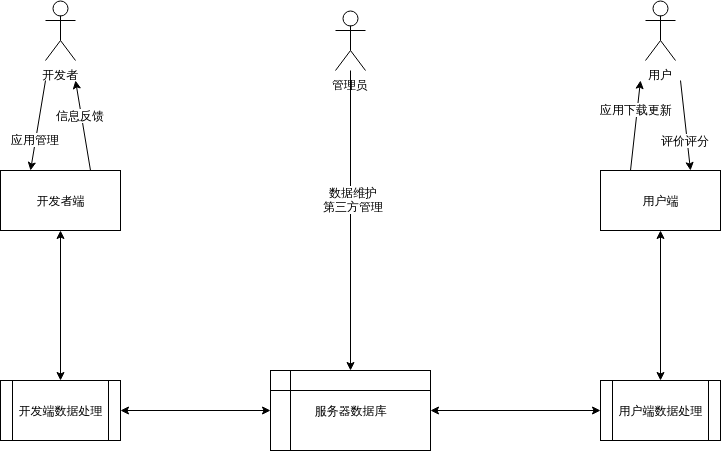
\includegraphics[width=10cm]{top_diagram.png}
	\caption{高层数据流图} \label{fig:top_diagram}
\end{figure}

下面的高层数据流图\ref{fig:top_diagram}简明扼要地说明了三个不同端之间的关系。


\section{用户特征}
开发者应该具有基本的开发能力,任何语言均可,本系统提供不同语言体系的打包与封装。

系统管理员应该具有基本的数据库维护能力。第三方的监督与广告投放应该交由管理员处理。

用户不假设具有任何的专业背景,要求是任何人均可以作为用户来使用本软件系统。


\section{假设和依赖关系}
本项目仅做最基本的假设,依赖于浏览器、网络协议、数据库以及具体的终端设备操作系统。

本项目尽可能面向未来,因而主要使用浏览器作为终端用户的交互设备,所以浏览器协议以及网络协议的改变
会对本项目造成影响。同时,鉴于部分用户的习惯依赖性,也需要提供相应的应用终端。
这一点需要考虑到不同PC或者手机的操作系统的架构。



\chapter{总体设计}
\section{软件描述}
系统包括服务器端、用户端和开发者端三个部分。

服务器端主要功能是:维护应用、开发者、用户的数据,响应和处理开发者端、用户端的请求,
提供管理人员管理接口,便于维护更新与第三方的接入。

用户端主要功能是:支持用户查询、下载、更新、安装、删除应用,并且能够对应用评价、评分。

开发者端端主要功能是:支持开发者上传、更新、删除应用,并且能够查询收入、将收入提现或转账、查询或回复应用的评价。

\section{处理流程}
\subsection{总体流程}
%overall_overall.png
\begin{figure}[ht]
	\centering
	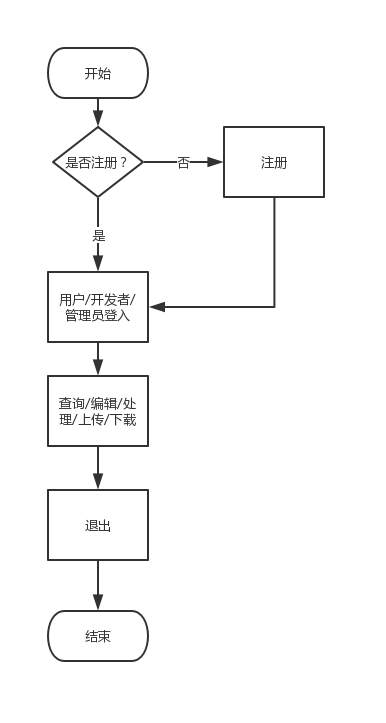
\includegraphics[width=8cm]{overall_overall.png}
	\caption{总体流程} \label{fig:overall_overall.png}
\end{figure}

总体流程针对使用者的逻辑。见图\ref{fig:overall_overall.png}

无论是开发者、用户还是管理员,都需要都账户,作为账户以及提供权限。

其中管理员的注册需要额外的信息以及身份验证。

\subsection{系统基本流程}
%overall_system.png
\begin{figure}[ht]
	\centering
	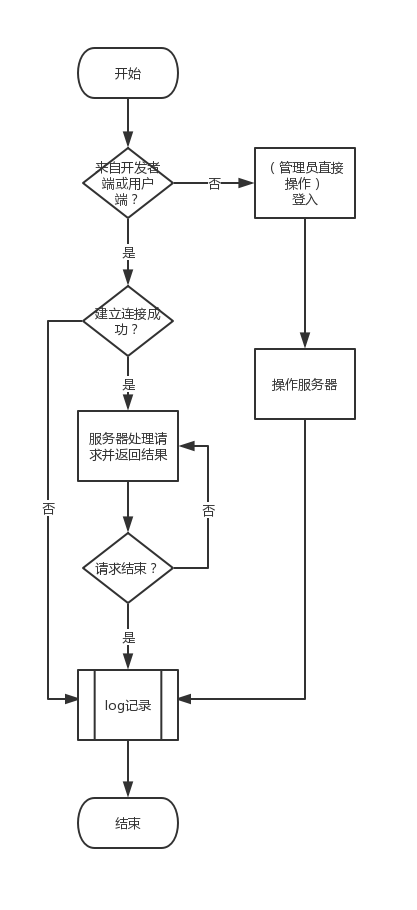
\includegraphics[width=10cm]{overall_system.png}
	\caption{系统基本流程} \label{fig:overall_system.png}
\end{figure}

系统基本流程简要表述不同的端与服务器的交互逻辑,见图\ref{fig:overall_system.png}.

主要需要区分管理人员和普通用户(包括应用开发人员)

普通用户是通过开发者端或者用户段软件与服务器进行连接,
然后请求通过网络交由服务器处理;而管理员需要使用另外的专门的接口,通过命令来操作。

\subsection{客户端基本流程}

我们之前提到过,不对开发者和普通用户用户作严格区分,两者共用一个客户端,开发者一定是普通用户,但反过来不成立。
\begin{figure}[ht]
	\centering
	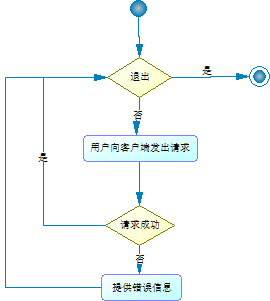
\includegraphics[width=6cm]{overall_client.png}
	\caption{客户端基本流程} \label{fig:overall_client.png}
\end{figure}
简单描述客户端处理用户请求的逻辑,见图\ref{fig:overall_client.png}

\subsection{客户端.注册与登录请求处理功能}
\begin{figure}[ht]
	\centering
	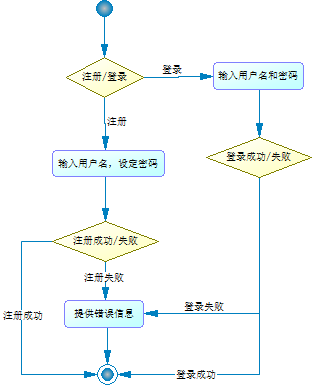
\includegraphics[width=10cm]{client_reg_login.png}
	\caption{客户端.注册与登录请求处理具体流程} \label{fig:client_reg_login.png}
\end{figure}

对于客户的登录与注册请求,见图\ref{fig:client_reg_login.png}

\subsection{客户端.普通用户应用管理请求处理功能}
\begin{figure}[ht]
	\centering
	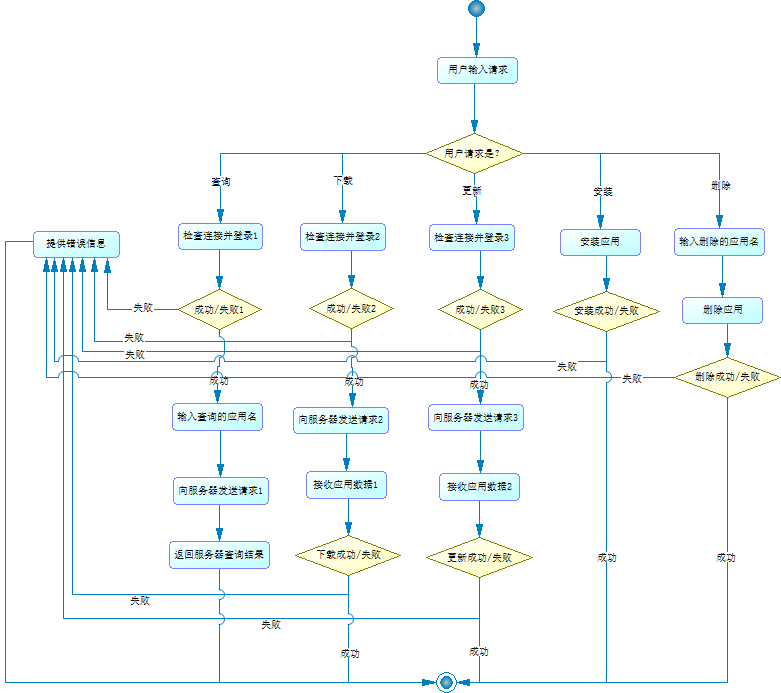
\includegraphics[width=16cm]{client_app.png}
	\caption{客户端.普通用户应用管理请求处理具体流程} \label{fig:client_app.png}
\end{figure}

对于客户的应用管理请求,见图\ref{fig:client_app.png}

\subsection{客户端.普通用户信息反馈请求处理功能}
\begin{figure}[ht]
	\centering
	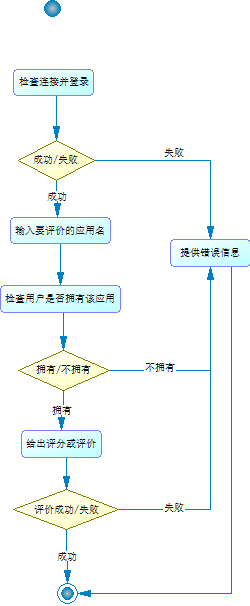
\includegraphics[width=8cm]{client_info.png}
	\caption{客户端.普通用户信息反馈处理具体流程} \label{fig:client_info.png}
\end{figure}

对于客户的信息反馈请求,见图\ref{fig:client_info.png}

\subsection{客户端.开发者应用管理请求处理功能}
\begin{figure}[ht]
	\centering
	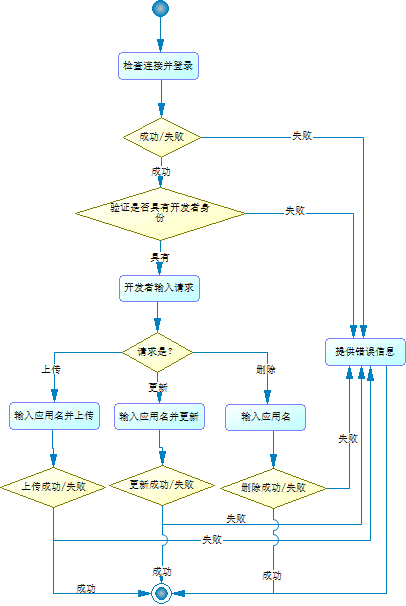
\includegraphics[width=10cm]{developer_app.png}
	\caption{客户端.开发者应用管理请求处理具体流程} \label{fig:developer_app.png}
\end{figure}

对于开发者的应用管理请求,见图\ref{fig:developer_app.png}

\subsection{客户端.开发者信息反馈请求处理功能}
\begin{figure}[ht]
	\centering
	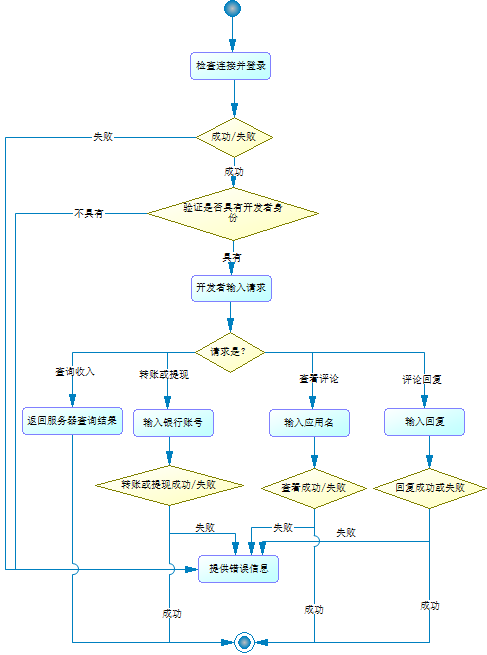
\includegraphics[width=12cm]{developer_info.png}
	\caption{客户端.开发者信息反馈请求处理具体流程} \label{fig:developer_info.png}
\end{figure}

对于开发者的信息反馈请求,见图\ref{fig:developer_info.png}


\subsection{服务器端基本流程}
%overall_sys.png
\begin{figure}[ht]
	\centering
	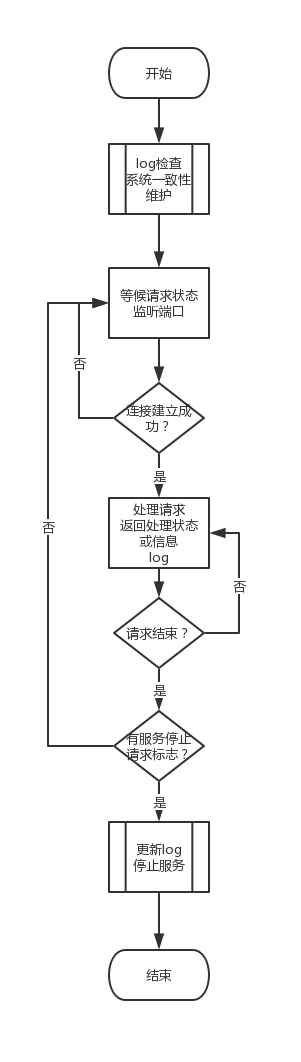
\includegraphics[width=6cm]{overall_sys.png}
	\caption{服务器端基本流程} \label{fig:overall_sys.png}
\end{figure}
简单描述服务器端处理请求的逻辑,见图\ref{fig:overall_sys.png}    .
注意管理员与服务器的交互也是通过网络连接的。
但是管理员没有相应的UI界面。


\subsection{服务器.注册与登录请求处理具体流程}
%overall_sys_login.png
\begin{figure}[ht]
	\centering
	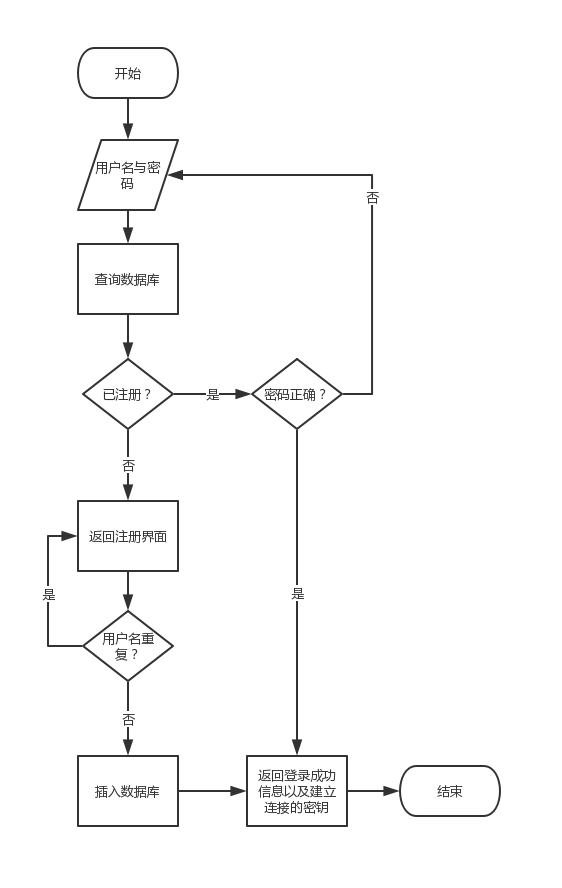
\includegraphics[width=12cm]{overall_sys_login.png}
	\caption{服务器.注册与登录请求处理具体流程} \label{fig:overall_sys_login.png}
\end{figure}

对于2类人员的登录与注册处理,见图\ref{fig:overall_sys_login.png}

此处的注册不包括管理员的注册,因为管理员的注册需要更多的权限,需要通过其他管理员添加进注册人员
列表。

\subsection{服务器.信息查询与修改请求处理具体流程}
%overall_sys_info.png
\begin{figure}[ht]
	\centering
	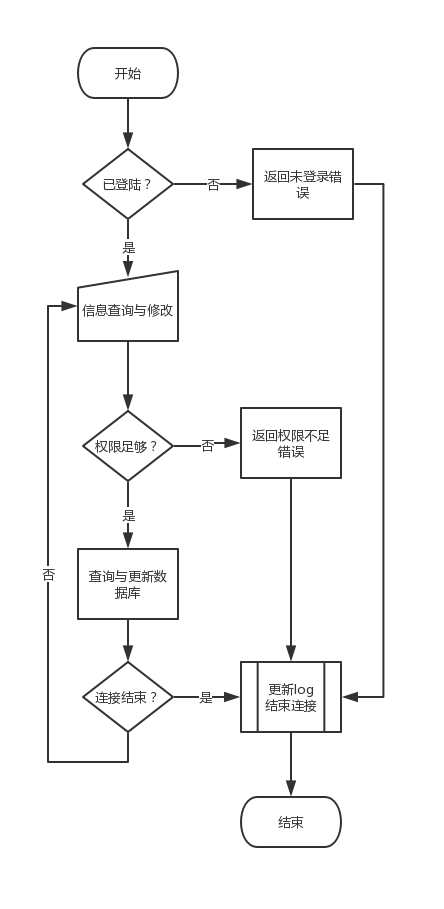
\includegraphics[width=10cm]{overall_sys_info.png}
	\caption{服务器.信息查询与修改请求处理具体流程} \label{fig:overall_sys_info.png}
\end{figure}

对于3类人员的信息查询与修改处理,见图\ref{fig:overall_sys_info.png}

修改需要额外的权限,比如非本app的开发人员不能修改该app的名称,简介等等。

\subsection{服务器.应用上传与下载请求处理具体流程}
%overall_sys_app.png
\begin{figure}[ht]
	\centering
	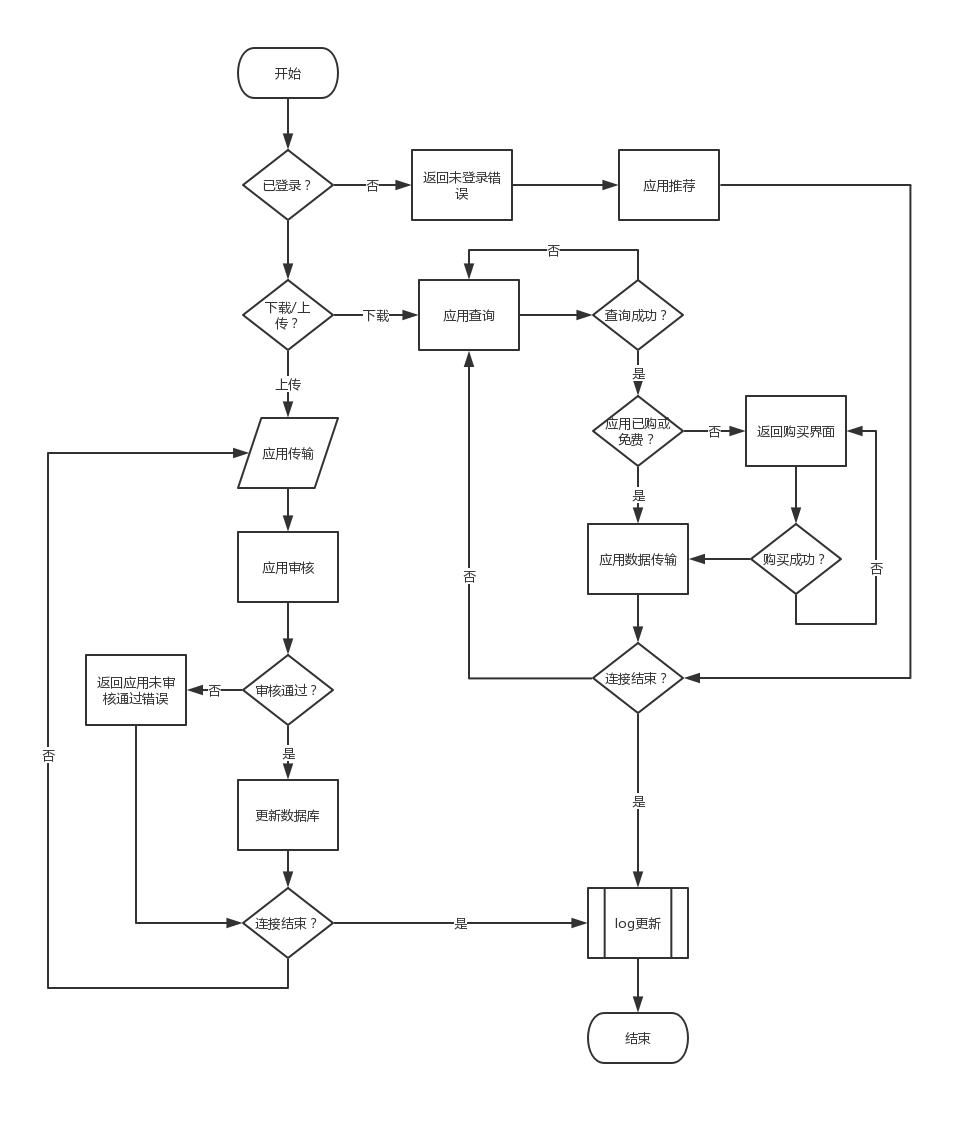
\includegraphics[width=16cm]{overall_sys_app.png}
	\caption{服务器.应用上传与下载请求处理具体流程} \label{fig:overall_sys_app.png}
\end{figure}

对于应用的上传与下载处理见图\ref{fig:overall_sys_app.png}.

上传有应用审核的要求,此处没有具体实现,同时搜索界面也有根据用户的习惯或者统计数据的
自动推荐功能。

\subsection{服务器.账户充值与提现请求处理具体流程}
%overall_sys_account.png
\begin{figure}[ht]
	\centering
	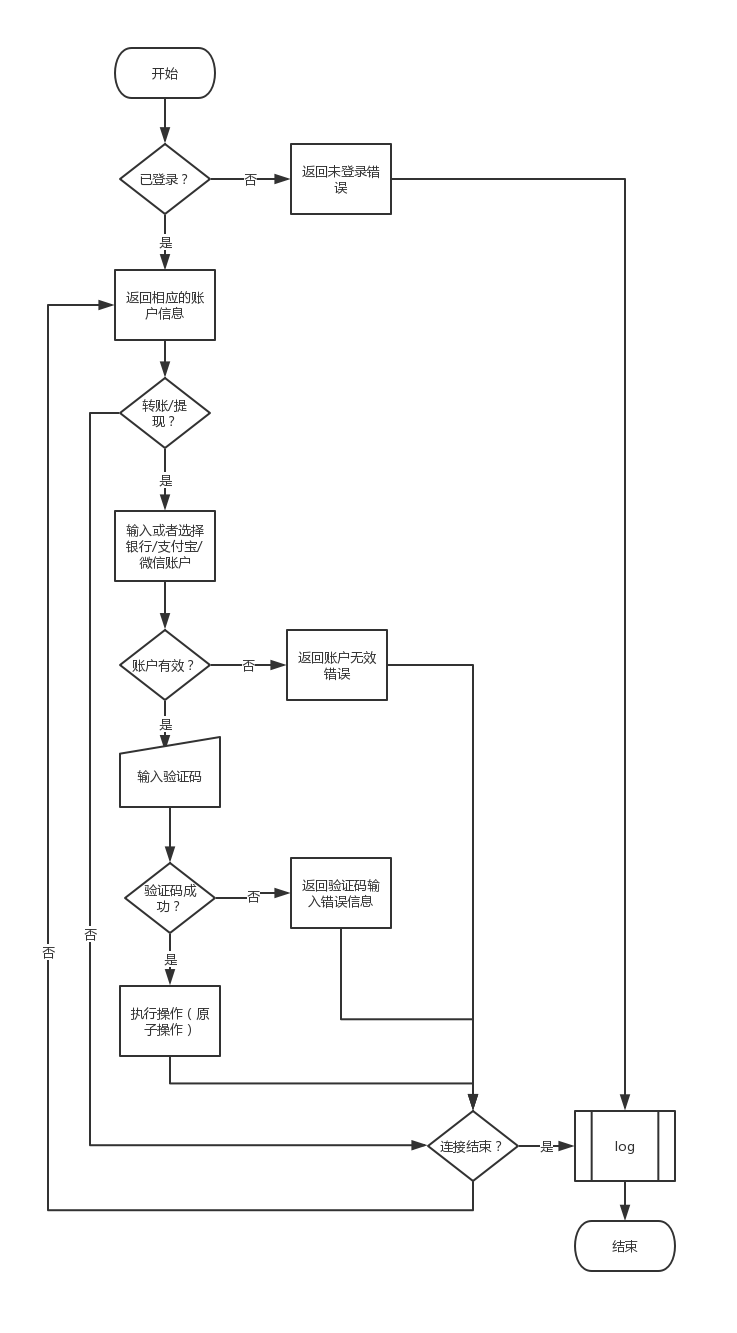
\includegraphics[width=13cm]{overall_sys_account.png}
	\caption{服务器.账户充值与提现请求处理具体流程} \label{fig:overall_sys_account.png}
\end{figure}

对于账户的管理见图\ref{fig:overall_sys_account.png}

可以添加不同的账户,这一点需要在后面提供统一的对外接口。

\subsection{服务器.应用信息查询与更新请求处理具体流程}
%overall_sys_app_info.png
\begin{figure}[ht]
	\centering
	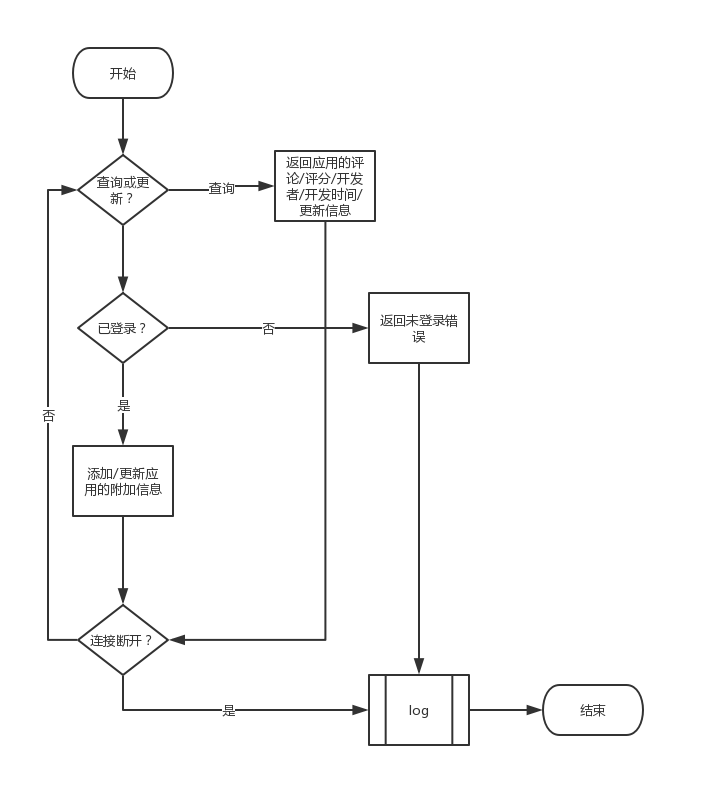
\includegraphics[width=14cm]{overall_sys_app_info.png}
	\caption{服务器.应用信息查询与更新请求处理具体流程} \label{fig:overall_sys_app_info.png}
\end{figure}

对应用的信息查询与评价、评分流程见\ref{fig:overall_sys_app_info.png}.

应用的信息主要针对某个app的评论与评分等等基本信息,与个人信息区分开。

\subsection{服务器.管理员操作请求处理具体流程}
%overall_sys_admin.png
\begin{figure}[ht]
	\centering
	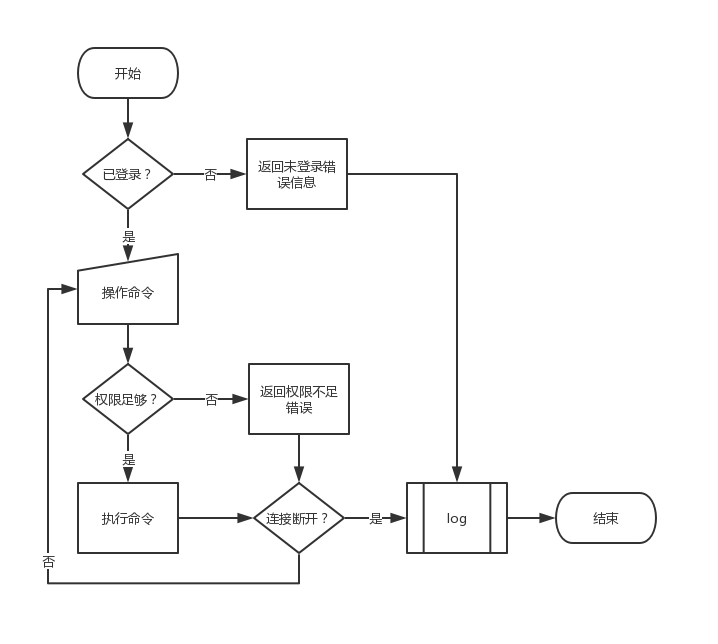
\includegraphics[width=14cm]{overall_sys_admin.png}
	\caption{服务器.管理员操作请求处理具体流程} \label{fig:overall_sys_admin.png}
\end{figure}

对于管理员级别的操作,见图\ref{fig:overall_sys_admin.png}

管理员直接通过命令行与服务器建立连接,同时需要检查每项操作的权限。

{\color{red}
\subsection{应用开发系统}
%overall_devsys.png
\begin{figure}[ht]
	\centering
	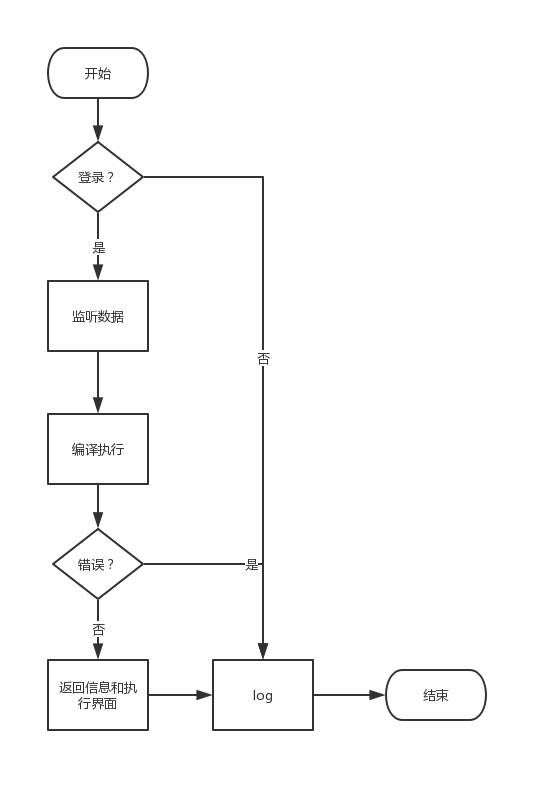
\includegraphics[width=10cm]{overall_devsys.png}
	\caption{服务器.管理员操作请求处理具体流程} \label{fig:overall_devsys.png}
\end{figure}


此处结合开发者端、服务器端、用户端,统一处理流程为图\ref{fig:overall_devsys.png}

}

\section{功能结构设计}
\subsection{整体结构}
%overall_structure0.png
\begin{figure}[ht]
	\centering
	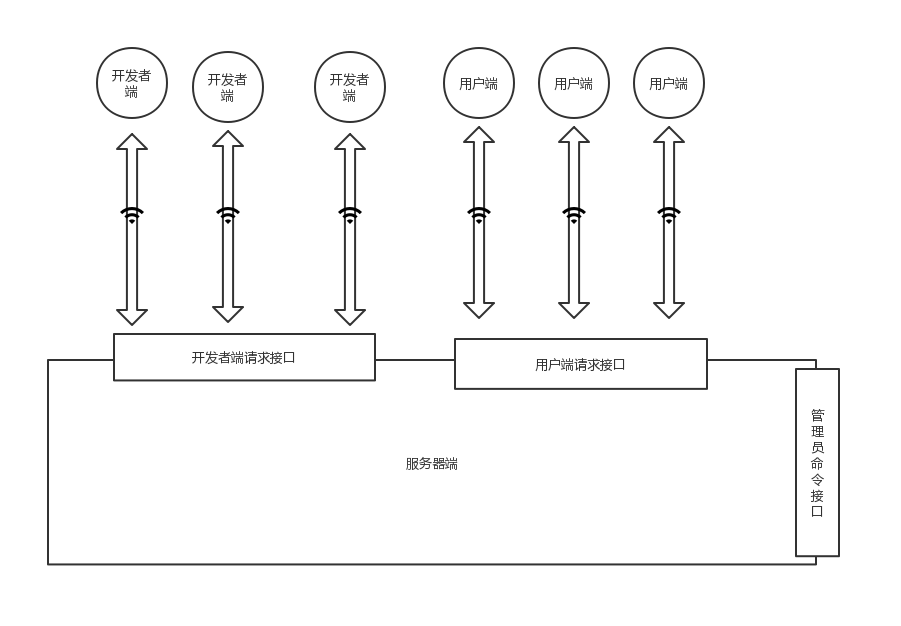
\includegraphics[width=16cm]{overall_structure0.png}
	\caption{整体结构} \label{fig:overall_structure0.png}
\end{figure}

整体结构见图\ref{fig:overall_structure0.png}

服务器端提供3种不同的对外接口,分别针对开发者、用户、管理员。


\subsection{客户端结构}
\begin{figure}[ht]
	\centering
	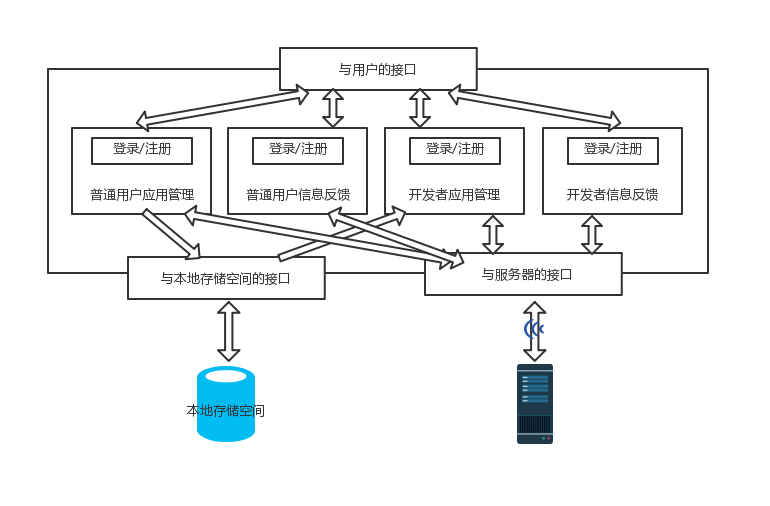
\includegraphics[width=12cm]{client_structure.png}
	\caption{客户端结构} \label{fig:client_structure}
\end{figure}

客户端的结构见图\ref{fig:client_structure}。

注意到,客户端可分为5个模块,其中注册/登录模块只会在其他模块中被调用,其他的模块相互独立。

\subsection{服务器端结构}
%overall_structure.png
\begin{figure}[ht]
	\centering
	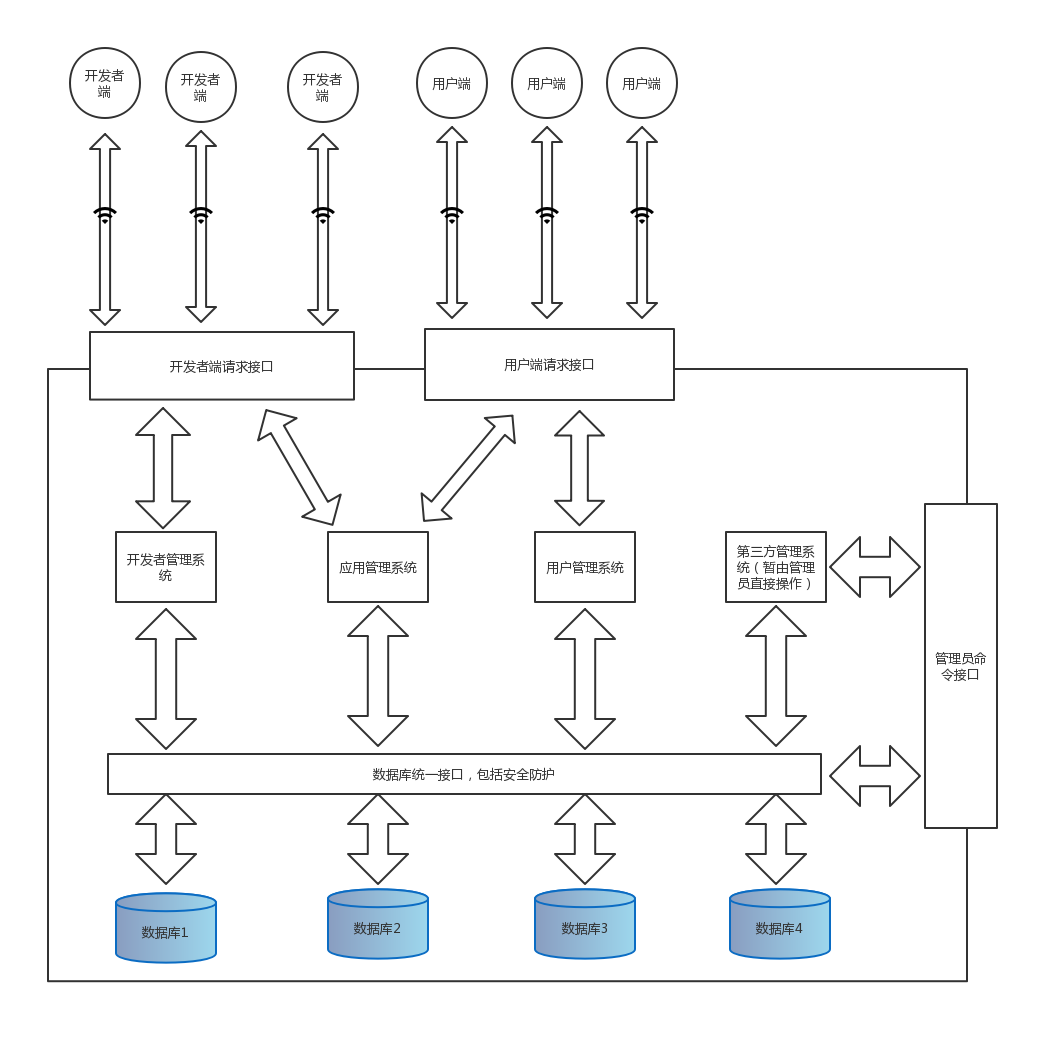
\includegraphics[width=16cm]{overall_structure.png}
	\caption{服务器端结构} \label{fig:overall_structure.png}
\end{figure}

服务器端结构见图\ref{fig:overall_structure.png}

服务器端的内部储存采用数据库,分布且冗余,避免物理失效。

为了安全起见,对外统一有数据库统一接口,接口的修改只能是最高权限的管理员。

普通管理员对外接口也是通过数据库统一接口操作的,同时兼任第三方管理系统的管理员。


\section{功能需求与程序代码的关系}
[此处指的是不同的需求分配到哪些模块去实现。可按不同的端拆分此表]
\begin{table}[htbp]
\centering
\caption{功能需求与程序代码的关系表} \label{tab:requirement-module}
\begin{tabular}{|c|c|c|c|c|c|}
    \hline
    需求编码 & 需求名称 & 开发者端应用管理模块 & 开发者端信息反馈模块 & 客户端应用管理模块 & 客户端信息反馈模块\\
    \hline
    SRS\_Dev\_App\_P01 & 开发者端.应用管理 & Y & · & . & .\\
    \hline
    SRS\_Dev\_Info\_P01 & 开发者端.信息反馈 & . & Y & . & .\\
    \hline
    SRS\_User\_App\_P01 & 客户端.应用管理 & . & · & Y & .\\
    \hline
    SRS\_User\_Info\_P01 & 客户端.信息反馈 & · & · & . & Y\\
    \hline
\end{tabular}
\note{各项功能需求的实现与各个程序模块的分配关系}
\end{table}
\chapter{接口设计}
\section{外部接口}

\subsection{账户接口}
账户的接口应该可以包括常见的电子账户,比如支付宝、微信、银行卡、Paypal等等,
在服务器内部形成统一的接口。需要实现的功能包括:电子账户添加、电子账户认证、
电子账户余额查询、电子账户充值到商店虚拟账户、商店虚拟账户转账到电子账户。

提供给内部的接口应该针对开发者管理系统和用户管理系统。

{\color{red}
	接口的具体定义为
	
\begin{lstlisting}[language=C, caption=账户接口, label={code:first-code}]
{
	string username //用户名
	string passwd //密码
	string account //账户
	vector<int> code //验证码
	float money //转账金额
	int error //错误码
}
\end{lstlisting}
}


\subsection{安装/卸载接口}
该接口用于客户端安装或卸载某个应用,只需提供该应用的安装/卸载程序的文件描述符或文件路径以及安装目录(如果是安装的话)即可。

{\color{red}
	接口的具体定义为
	
\begin{lstlisting}[language=C, caption=安装/卸载接口, label={code:first-code}]
{
	string username //用户名
	vector<int> code //验证码
	string file //文件路径
}	
\end{lstlisting}
}

\subsection{用户接口}
用户接口分为提供给普通用户和开发者的接口。

提供给普通用户的接口包括登录、注册、应用查询、应用购买、应用安装、应用删除、应用评分等等。

提供给开发者的接口包括登录、注册、应用上传、应用更新、应用删除、收入查询、转账提现、评论查看、评论回复等等。

分别参见表\ref{tab:developer_interface}和表\ref{tab:client_interface}。

\begin{longtable}{|p{4cm}|p{5cm}|p{5cm}|}
	\caption{开发者与应用商店系统的接口}\label{tab:developer_interface} \\
	\hline
	\textbf{开发者需求} & \textbf{输入} & \textbf{输出}\\
	\hline
	\endfirsthead
	\hline
	\textbf{开发者需求} & \textbf{输入} & \textbf{输出}\\
	\hline
	\endhead
	\hline 
	\endfoot
	\hline
	\endlastfoot
	登录 & 账号、密码 & 登录成功与否\\
	注册 & 账号、密码 & 注册成功与否\\
	应用上传 & 本地应用 & 上传成功与否\\
	应用更新 & 本地应用和待更新应用id & 更新成功与否\\
	应用删除 & 待删除应用id & 删除成功与否\\
    收入查询 & 无 & 收入\\
    转账提现 & 银行账号 & 转账或提现成功与否\\
	评论回复 & 回复内容 & 回复成功与否\\
	\end{longtable}

\begin{longtable}{|p{4cm}|p{5cm}|p{5cm}|}
	\caption{普通用户与应用商店系统的接口}\label{tab:client_interface} \\
	\hline
	\textbf{用户需求} & \textbf{输入} & \textbf{输出}\\
	\hline
	\endfirsthead
	\hline
	\textbf{用户需求} & \textbf{输入} & \textbf{输出}\\
	\hline
	\endhead
	\hline 
	\endfoot
	\hline
	\endlastfoot
	登录 & 账号、密码 & 登录成功与否\\
	注册 & 账号、密码 & 注册成功与否\\
	应用查询 & 应用id & 相关的应用,以列表呈现\\
	应用购买 & 待购买应用id和银行账户 & 购买成功与否\\
	应用安装 & 待安装应用id & 安装成功与否\\
    应用删除 & 待删除应用id & 删除成功与否\\
	应用评分 & 待评价应用id和评分 & 评分成功与否\\
	应用评价 & 待评价应用id和评论 & 评论成功与否\\
	\end{longtable}

用户接口最终将以图形界面呈现。


{\color{red}
	接口的具体定义为
	
\begin{lstlisting}[language=C, caption=安装/卸载接口, label={code:first-code}]
{
	string username //用户名
	string passwd //密码
	string command //指令
	string permission //权限等级
}
\end{lstlisting}
}

\section{内部接口}

\subsection{客户端}
如第三章的描述,客户端主要有这几个模块:注册或登录模块、普通用户应用管理模块、普通用户信息反馈模块、开发者应用管理模块、开发者信息反馈模块。

后面4个模块相对独立,相互之间没有交互。注册或登录模块会作为子模块被后面4个模块调用。


{\color{red}
	接口的具体定义为
	
\begin{lstlisting}[language=C, caption=安装/卸载接口, label={code:first-code}]
{
	vector<int> number //终端编码
	vector<int> code //验证码
	int command //指令编号
	data_type data //数据
}
\end{lstlisting}
}

\subsection{服务器端与数据库}
服务器端内部提供数据库统一接口,提供给开发者管理系统、应用管理系统、用户管理系统、第三方管理系统
使用,目的是提高安全性与简便。

提供高阶的增删改查接口,不需要直接使用PL/SQL.

不同的功能需要有不同的权限,比如修改删除需要的权限高于查询,同时,只有管理员才有直接使用PL/SQL查询
的权限。另外,应该提供方便的增加高阶功能的接口。


{\color{red}
	接口的具体定义为
	
\begin{lstlisting}[language=C, caption=安装/卸载接口, label={code:first-code}]
{
	vector<int> number //服务器编码
	vector<int> code //验证码
	int permission //权限等级
	string command //指令
	data_type data //数据
}
\end{lstlisting}
}
\chapter{数据结构设计}
\section{逻辑结构设计}
\subsection{客户端数据结构}
客户端在运行过程中,需要维护的信息如下:

生命周期为整个程序运行过程的信息有:

\begin{itemize}
    \item 用户名,如果尚未登录则为空
    \item 当前请求
    \item 请求结果
\end{itemize}

生命周期为某个请求处理过程的信息有:

\begin{enumerate}
    \item 普通用户应用管理:数据结构1\\
        \begin{itemize}
            \item 目标应用名
        \end{itemize}
    \item 普通用户信息反馈:数据结构2\\
        \begin{itemize}
            \item 目标应用名
            \item 评价或评分
        \end{itemize}
    \item 开发者应用管理:数据结构3\\
        \begin{itemize}
            \item 目标应用名
        \end{itemize}
    \item 开发者信息反馈:数据结构4\\
        \begin{itemize}
            \item 目标应用名
            \item 回复的评论
            \item 银行账号
        \end{itemize}
\end{enumerate}

根据具体的请求,以上的数据结构还可再进一步细化。

\subsection{服务器端数据结构}
数据部分使用Oracle数据库存储,并不需要特别的数据结构。

\section{物理结构设计}
各数据结构无特殊物理结构要求。

\section{数据结构与程序模块的关系}
[此处指的是不同的数据结构分配到哪些模块去实现。可按不同的端拆分此表]
\begin{table}[htbp]
\centering
\caption{数据结构与程序代码的关系表} \label{tab:datastructure-module}
\begin{tabular}{|c|c|c|c|c|}
    \hline
    · & 普通用户应用管理 & 普通用户信息反馈 & 开发者应用管理 & 开发者信息反馈\\
    \hline
    数据结构1 & Y & · & · & ·\\
    \hline
    数据结构2 & · & Y & · & ·\\
    \hline
    数据结构3 & · & · & Y & ·\\
    \hline
    数据结构4 & · & · & · & Y\\
    \hline
\end{tabular}
\note{各项数据结构的实现与各个程序模块的分配关系}
\end{table}
\chapter{数据库设计}
\section{数据库环境说明}
{\color{red}
\subsection{检索速度v.s.稳定性}
本应用并不强调检索的速度,因为应用的数量并不会过多,所以更多地从稳定性考虑。

    从稳定性考虑,本系统的数据系统采用Oracle 12数据库系统;使用centOS作为
    操作系统。

\subsection{数据一致性考虑}
本系统同时也不强调一致性,应用的开发、应用的下载并不是冲突的操作。

用户下载的应用仅仅是系统中的最新版本即可。

}



\section{数据库的命名规则}
允许单词缩写,缩写的要求见表\ref{tab:abbr}

表名为单数,当前阶段设计的表有app,user,developer,people,dev\_app,user\_own\_app,comment.

字段无需加上前缀


\section{逻辑设计}
\begin{figure}[ht]
	\centering
	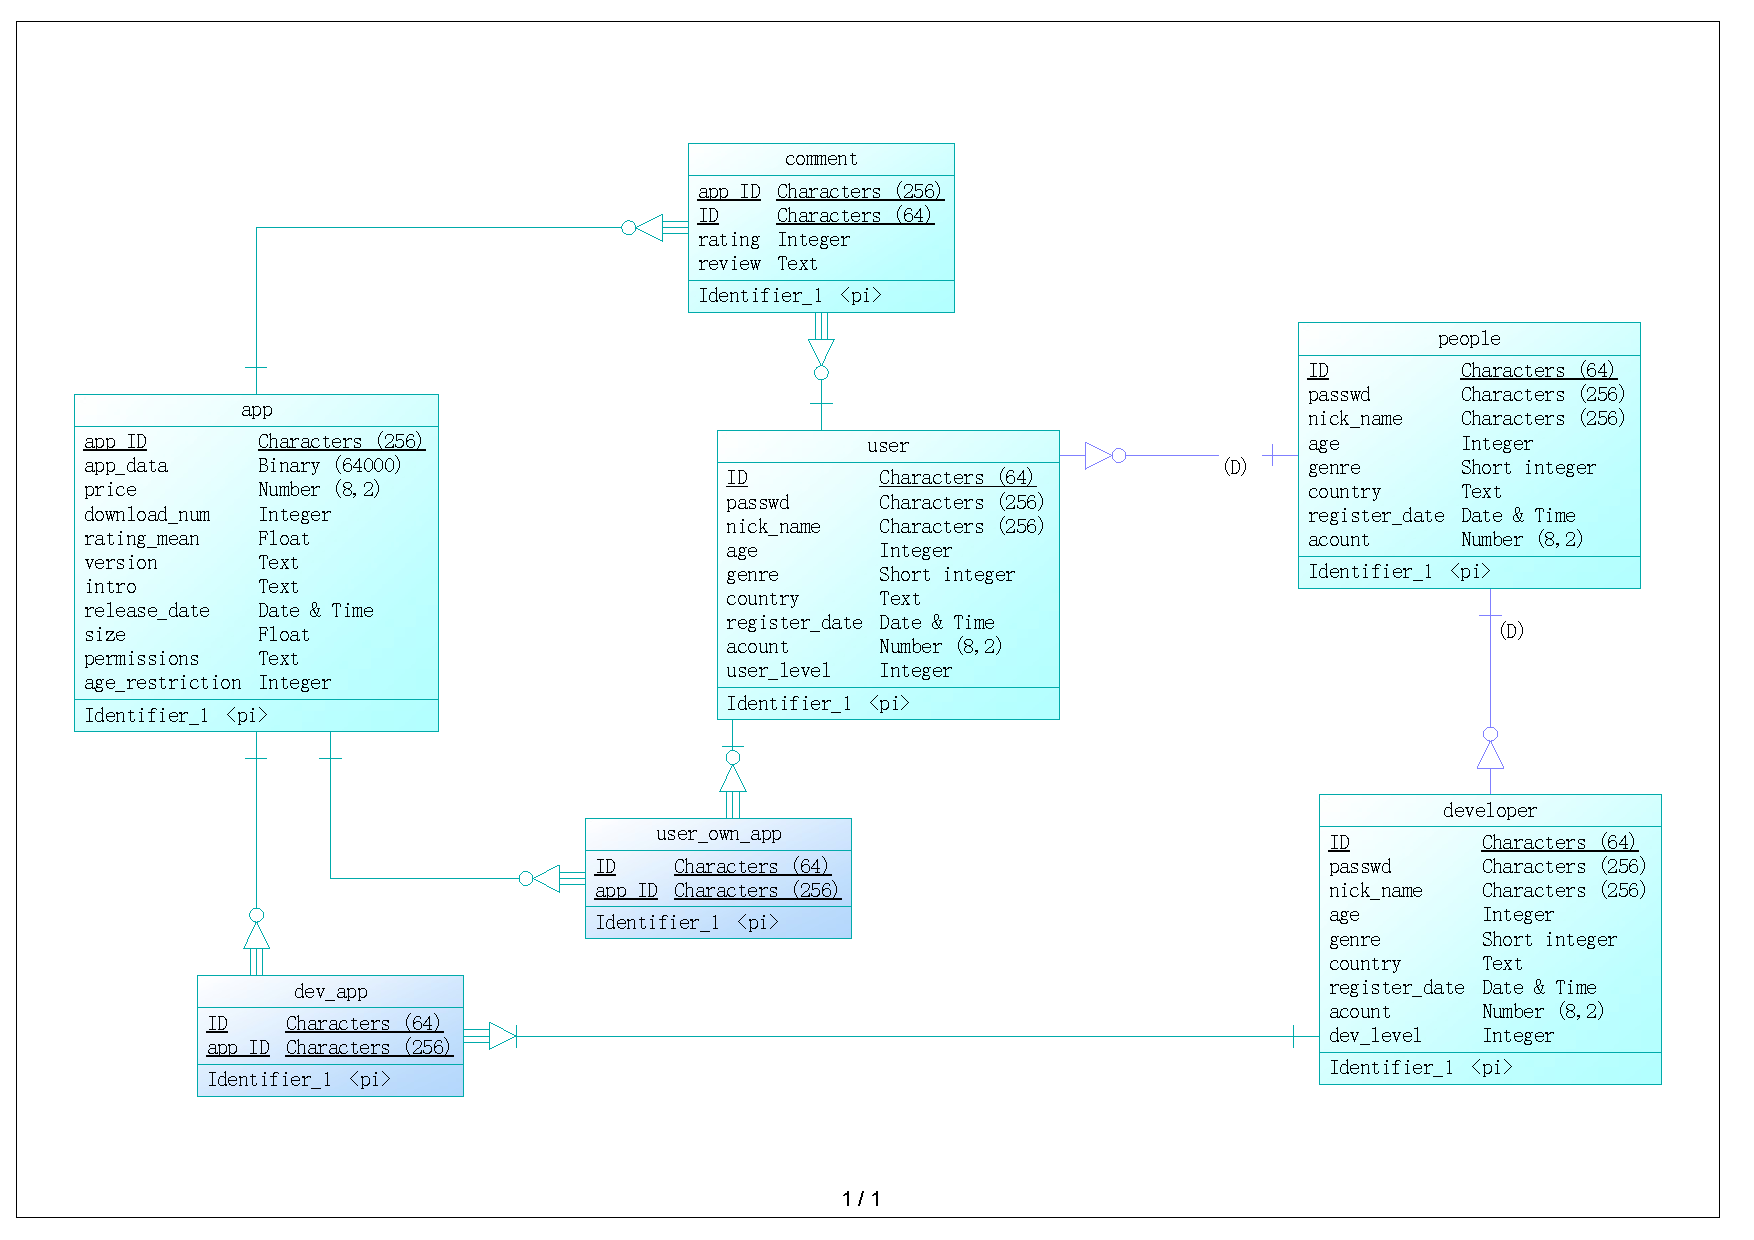
\includegraphics[width=16cm]{logical_data_model.pdf}
	\caption{逻辑模型图} \label{fig:logical_data_model.pdf}
\end{figure}
基本的实体关系逻辑模型见图\ref{fig:logical_data_model.pdf}



\section{物理设计}
\subsection{数据库产品}
使用oracle 12c数据库,要求是分布的且冗余。

\subsection{实体属性、类型、精度}
\subsubsection{app数据表设计}
\begin{table}[htbp]
\centering
\caption{app数据表Users设计} \label{tab:app_database}
\begin{tabular}{|c|c|c|c|c|}
    \hline
    字段名 & 类型 & 大小 & 说明 & 备注 \\
    \hline
    app\_ID & char & 256 & app的全局唯一标识符 & 主键 \\
    \hline
    app\_data & binary & $\cdot$ & app数据 & $\cdot$ \\
    \hline
    price & number & $\cdot$ & app的价格 & $\cdot$ \\
    \hline
    download\_num & int & $\cdot$ & 下载数量 & $\cdot$ \\
    \hline 
    rating\_mean & float & $\cdot$ & 平均评分 & $\cdot$ \\
    \hline
    version & text & $\cdot$ & 版本号 & $\cdot$ \\
    \hline
    intro & text & $\cdot$ & 简介 & $\cdot$ \\
    \hline
    release\_date & Date \& Time & $\cdot$ & 发行时间 & $\cdot$ \\
    \hline
    size & float & $\cdot$ & app数据大小 & $\cdot$ \\
    \hline 
    permissions & text & $\cdot$ & 权限要求 & $\cdot$ \\
    \hline
    age\_restriction & int & $\cdot$ & 用户年龄限制 & $\cdot$ \\
    \hline
\end{tabular}
%\note{用户数据表Users设计}
\end{table}

app表设计见图\ref{tab:app_database}

\subsubsection{user数据表设计}
\begin{table}[htbp]
\centering
\caption{user数据表设计} \label{tab:user_database}
\begin{tabular}{|c|c|c|c|c|}
    \hline
    字段名 & 类型 & 大小 & 说明 & 备注 \\
    \hline
    ID & char & 64 & 人员ID & 主键 \\
    \hline
    passwd & char & 256 & 加密后的密码 & $\cdot$ \\
    \hline
    nick\_name & char & 256 & 昵称 & $\cdot$ \\
    \hline 
    age & int & $\cdot$ & 年龄 & 考虑到年龄限制 \\
    \hline
    genre & char & 1 & 性别 & $\cdot$ \\
    \hline
    country & text & $\cdot$ & 国家 & 考虑到地域限制 \\
    \hline
    register\_date & Date\& Time & $\cdot$ & 注册时间 & $\cdot$ \\
    \hline
    acount & number & $\cdot$ & 账户金额 & $\cdot$ \\
    \hline
    user\_level & int & $\cdot$ & 用户的等级 & $\cdot$ \\
    \hline
\end{tabular}
%\note{订单数据表Orders设计}
\end{table}
user数据表设计见图\ref{tab:user_database}

\subsubsection{developer数据表设计}
\begin{table}[htbp]
\centering
\caption{developer数据表设计} \label{tab:developer_database}
\begin{tabular}{|c|c|c|c|c|}
    \hline
    字段名 & 类型 & 大小 & 说明 & 备注 \\
    \hline
    ID & char & 64 & 人员ID & 主键 \\
    \hline
    passwd & char & 256 & 加密后的密码 & $\cdot$ \\
    \hline
    nick\_name & char & 256 & 昵称 & $\cdot$ \\
    \hline 
    age & int & $\cdot$ & 年龄 & 考虑到年龄限制 \\
    \hline
    genre & char & 1 & 性别 & $\cdot$ \\
    \hline
    country & text & $\cdot$ & 国家 & 考虑到地域限制 \\
    \hline
    register\_date & Date\& Time & $\cdot$ & 注册时间 & $\cdot$ \\
    \hline
    acount & number & $\cdot$ & 账户金额 & $\cdot$ \\
    \hline
    dev\_level & int & $\cdot$ & 开发者的等级 & $\cdot$ \\
    \hline
\end{tabular}
%\note{订单数据表Orders设计}
\end{table}
developer数据表设计见表\ref{tab:developer_database}

\subsubsection{comment数据表设计}
\begin{table}[htbp]
\centering
\caption{comment数据表设计} \label{tab:comment_database}
\begin{tabular}{|c|c|c|c|c|}
    \hline
    字段名 & 类型 & 大小 & 说明 & 备注 \\
    \hline
    app\_ID & char & 256 & app的标识符 & 外键,来自app表\\
    \hline
    ID & char & 64 & 人员的ID & 外键,来自user表 \\
    \hline 
    rating & int & $\cdot$ & 评分& 0-5 \\
    \hline
    review & text & $\cdot$ & 评论 & $\cdot$ \\
    \hline
\end{tabular}
%\note{订单数据表Orders设计}
\end{table}
评论、评分数据表设计见表\ref{tab:comment_database}


\subsubsection{dev\_app数据表设计}
\begin{table}[htbp]
\centering
\caption{dev\_app数据表设计} \label{tab:dev_app_database}
\begin{tabular}{|c|c|c|c|c|}
    \hline
    字段名 & 类型 & 大小 & 说明 & 备注 \\
    \hline
    app\_ID & char & 256 & app的标识符 & 外键,来自app表\\
    \hline
    ID & char & 64 & 人员的ID & 外键,来自user表 \\
    \hline 
\end{tabular}
%\note{订单数据表Orders设计}
\end{table}
开发者开发的app表设计见表\ref{tab:dev_app_database}

\subsubsection{user\_own\_app数据表设计}
\begin{table}[htbp]
\centering
\caption{user\_own\_app数据表设计} \label{tab:user_own_app_database}
\begin{tabular}{|c|c|c|c|c|}
    \hline
    字段名 & 类型 & 大小 & 说明 & 备注 \\
    \hline
    app\_ID & char & 256 & app的标识符 & 外键,来自app表\\
    \hline
    ID & char & 64 & 人员的ID & 外键,来自user表 \\
    \hline 
\end{tabular}
%\note{订单数据表Orders设计}
\end{table}
用户拥有的(已购买或者已下载的)app表设计见表\ref{tab:user_own_app_database}

\section{安全性设计}
备份和容灾设计。

\section{数据库管理与维护说明}
对于数据库的维护,随时对数据库中的信息加以调试和保存备份。同样需要个工作人员进行系统的分析和用户的反馈,对系统进行升级以及功能的完善。同时保证系统安全有序的运行。
\chapter{界面设计}
\section{客户端界面}
之前已经多次提到过,普通用户和开发者共用一个客户端。

界面示例见图\ref{fig:ui_desktop_home}、\ref{fig:ui_desktop_app}、\ref{fig:ui_mobile_home}、\ref{fig:ui_mobile_app}。

\begin{figure}[ht]
	\centering
	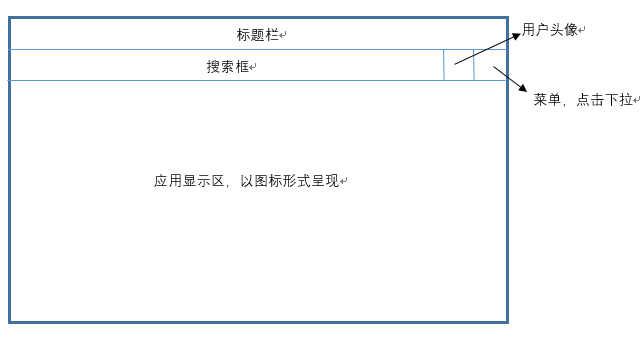
\includegraphics[width=10cm]{ui_desktop.png}
	\caption{桌面端应用商店主界面} \label{fig:ui_desktop_home}
\end{figure}

\begin{figure}[ht]
	\centering
	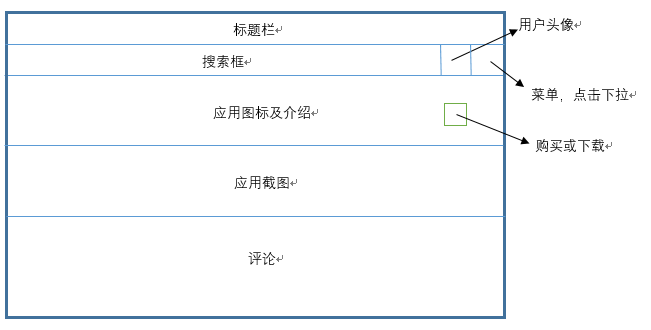
\includegraphics[width=10cm]{ui_desktop1.png}
	\caption{桌面端应用商店应用界面} \label{fig:ui_desktop_app}
\end{figure}

\begin{figure}[ht]
	\centering
	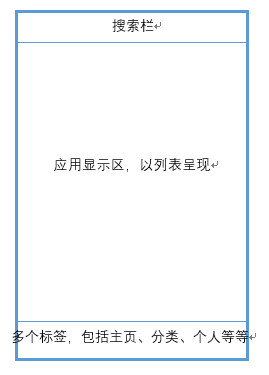
\includegraphics[width=6cm]{ui_mobile.png}
	\caption{移动端应用商店主界面} \label{fig:ui_mobile_home}
\end{figure}

\begin{figure}[ht]
	\centering
	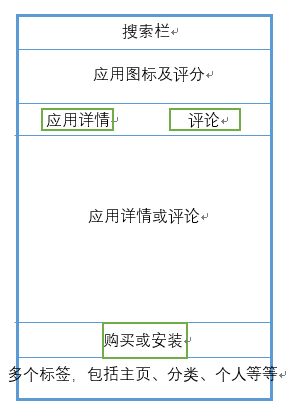
\includegraphics[width=6cm]{ui_mobile1.png}
	\caption{移动端应用商店应用界面} \label{fig:ui_mobile_app}
\end{figure}

以上只列出了部分用户界面。最终的用户界面可能与目前的示例有所偏差。

\section{服务器端界面}
服务器端不需要界面。管理员直接使用命令行交互。


\chapter{出错处理设计}

\section{客户端出错处理}
客户端的错误可以分为两类:由于网络异常导致的和服务器通信中断、用户发出的请求未能得到满足。

第一类错误应提醒用户检查网络状态,第二类错误是因为用户不具备完成其请求的条件,如试图评价一个用户不拥有的应用,
此类错误由服务器返回,提醒用户重新操作即可。

另外,客户端可能会由于未知的原因而崩溃,对于这类问题可以设置一个日志来存储客户端的行为,以便重启客户端后进行恢复以及
向服务器发送崩溃记录,但也可不做处理,因为应用商店不是类似办公软件的程序,不会涉及到具有很大价值的数据。

\section{服务器端出错处理}
服务器有两种避免重大错误的方式,一是使用log, 二是数据库采用分布式冗余设计。

紧急错误出现时,立即停止系统,并且上线备份系统。

通常的错误可以使用log自动或者人工修正,管理员可以添加自动修正规则。

非常重大的人为错误或者物理失效,仍然有分布式冗余的数据库作为保证。
\chapter{安全保密设计}
\section{客户端安全设计}
客户端涉及的重要数据只有用户名和密码以及银行账号。

可以对这些信息加密传输,具体方法如下:

\begin{enumerate}
\item 服务器端通过RSA公钥加密系统生成一对公钥和私钥,并将公钥派发给客户端。
\item 客户端在传输上述重要信息前,首先生成一个对称密钥。
\item 客户端使用服务器的公钥对生成的对称密钥加密,然后发送给服务器。
\item 服务器使用私钥对收到的信息解密,得到客户端的对称密钥。
\item 客户端和服务器可以通过对称密钥进行通信。
\end{enumerate}

\section{服务器端安全设计}
最重要的数据在数据库,所以最关键的安全防护在于数据库统一接口,避免人为失误,
同时也能避免网络攻击。

同时另一个是用户端接口和开发者端接口,即暴露给外面的接口有限,而且经过严格的设计与攻击检测。
\chapter{维护设计}
\section{客户端维护}
客户端需要记录的信息只有:已安装应用及其卸载程序路径、已下载但未安装的应用安装程序路径。

\section{服务器端维护}
所有不符合常规的错误都会形成log定期发送给管理员。

同时每隔固定的时间检测整个系统的稳定性。

%\chapter{图片}
本章展示图片相关用法。

\section{示例}
\begin{figure}[ht]
\centering

\includegraphics[width=10cm]{ustc_logo_fig}
\caption{测试图片} \label{fig:figure1}
\end{figure}

\section{带图注的图}
\begin{figure}[ht]
\centering

\includegraphics[width=10cm]{ustc_logo_fig}
\caption{带图注的图片}\label{fig:noted-figure}
\note{the solid lines represent the time histogram of the spontaneous activities of an old monkey cell(gray) and a young monkey cell (black). The bin-width is 1}
\end{figure}

%\chapter{表格}

\section{A Simple Table}
\begin{table}[htbp]
\centering
\caption{这里是表的标题} \label{tab:simpletable}
\begin{tabular}{|c|c|}
    \hline
    a & b \\
    \hline
    c & d \\
    \hline
\end{tabular}
\note{这里是表的注释}
\end{table}

\section{长表格}
\begin{longtable}{ccc}
% 首页表头
\caption[长表格演示]{长表格演示} \label{tab:longtable} \\
\toprule[1.5pt]
名称  & 说明 & 备注\\
\midrule[1pt]
\endfirsthead
% 续页表头
\caption[]{长表格演示(续)} \\
\toprule[1.5pt]
名称  & 说明 & 备注 \\
\midrule[1pt]
\endhead
% 首页表尾
\hline
\multicolumn{3}{r}{\small 续下页}
\endfoot
% 续页表尾
\bottomrule[1.5pt]
\endlastfoot

AAAAAAAAAAAA   &   BBBBBBBBBBB   &   CCCCCCCCCCCCCC   \\
AAAAAAAAAAAA   &   BBBBBBBBBBB   &   CCCCCCCCCCCCCC   \\
AAAAAAAAAAAA   &   BBBBBBBBBBB   &   CCCCCCCCCCCCCC   \\
AAAAAAAAAAAA   &   BBBBBBBBBBB   &   CCCCCCCCCCCCCC   \\
AAAAAAAAAAAA   &   BBBBBBBBBBB   &   CCCCCCCCCCCCCC   \\
AAAAAAAAAAAA   &   BBBBBBBBBBB   &   CCCCCCCCCCCCCC   \\
AAAAAAAAAAAA   &   BBBBBBBBBBB   &   CCCCCCCCCCCCCC   \\
AAAAAAAAAAAA   &   BBBBBBBBBBB   &   CCCCCCCCCCCCCC   \\
AAAAAAAAAAAA   &   BBBBBBBBBBB   &   CCCCCCCCCCCCCC   \\
AAAAAAAAAAAA   &   BBBBBBBBBBB   &   CCCCCCCCCCCCCC   \\
AAAAAAAAAAAA   &   BBBBBBBBBBB   &   CCCCCCCCCCCCCC   \\
AAAAAAAAAAAA   &   BBBBBBBBBBB   &   CCCCCCCCCCCCCC   \\
AAAAAAAAAAAA   &   BBBBBBBBBBB   &   CCCCCCCCCCCCCC   \\
AAAAAAAAAAAA   &   BBBBBBBBBBB   &   CCCCCCCCCCCCCC   \\
AAAAAAAAAAAA   &   BBBBBBBBBBB   &   CCCCCCCCCCCCCC   \\
AAAAAAAAAAAA   &   BBBBBBBBBBB   &   CCCCCCCCCCCCCC   \\
AAAAAAAAAAAA   &   BBBBBBBBBBB   &   CCCCCCCCCCCCCC   \\
AAAAAAAAAAAA   &   BBBBBBBBBBB   &   CCCCCCCCCCCCCC   \\
AAAAAAAAAAAA   &   BBBBBBBBBBB   &   CCCCCCCCCCCCCC   \\
AAAAAAAAAAAA   &   BBBBBBBBBBB   &   CCCCCCCCCCCCCC   \\
AAAAAAAAAAAA   &   BBBBBBBBBBB   &   CCCCCCCCCCCCCC   \\
AAAAAAAAAAAA   &   BBBBBBBBBBB   &   CCCCCCCCCCCCCC   \\
AAAAAAAAAAAA   &   BBBBBBBBBBB   &   CCCCCCCCCCCCCC   \\
AAAAAAAAAAAA   &   BBBBBBBBBBB   &   CCCCCCCCCCCCCC   \\
AAAAAAAAAAAA   &   BBBBBBBBBBB   &   CCCCCCCCCCCCCC   \\
AAAAAAAAAAAA   &   BBBBBBBBBBB   &   CCCCCCCCCCCCCC   \\
AAAAAAAAAAAA   &   BBBBBBBBBBB   &   CCCCCCCCCCCCCC   \\
AAAAAAAAAAAA   &   BBBBBBBBBBB   &   CCCCCCCCCCCCCC   \\
AAAAAAAAAAAA   &   BBBBBBBBBBB   &   CCCCCCCCCCCCCC   \\
AAAAAAAAAAAA   &   BBBBBBBBBBB   &   CCCCCCCCCCCCCC   \\
AAAAAAAAAAAA   &   BBBBBBBBBBB   &   CCCCCCCCCCCCCC   \\
AAAAAAAAAAAA   &   BBBBBBBBBBB   &   CCCCCCCCCCCCCC   \\
AAAAAAAAAAAA   &   BBBBBBBBBBB   &   CCCCCCCCCCCCCC   \\
AAAAAAAAAAAA   &   BBBBBBBBBBB   &   CCCCCCCCCCCCCC   \\
AAAAAAAAAAAA   &   BBBBBBBBBBB   &   CCCCCCCCCCCCCC   \\
AAAAAAAAAAAA   &   BBBBBBBBBBB   &   CCCCCCCCCCCCCC   \\
\end{longtable}

%\chapter{算法环境}
模板中使用 \texttt{algorithm2e} 宏包实现算法环境。关于该宏包的具体用法,
请阅读宏包的官方文档。

\begin{algorithm}[htbp]
\SetAlgoLined
\KwData{this text}
\KwResult{how to write algorithm with \LaTeX2e }

initialization\;
\While{not at end of this document}{
    read current\;
    \eIf{understand}{
        go to next section\;
        current section becomes this one\;
    }{
        go back to the beginning of current section\;
    }
}
\caption{算法示例1}
\label{algo:algorithm1}
\end{algorithm}

\IncMargin{1em}
\begin{algorithm}
\SetKwData{Left}{left}\SetKwData{This}{this}\SetKwData{Up}{up}
\SetKwFunction{Union}{Union}\SetKwFunction{FindCompress}{FindCompress}
\SetKwInOut{Input}{input}\SetKwInOut{Output}{output}

\Input{A bitmap $Im$ of size $w\times l$}
\Output{A partition of the bitmap}
\BlankLine
\emph{special treatment of the first line}\;
\For{$i\leftarrow 2$ \KwTo $l$}{
    \emph{special treatment of the first element of line $i$}\;
    \For{$j\leftarrow 2$ \KwTo $w$}{\label{forins}
        \Left$\leftarrow$ \FindCompress{$Im[i,j-1]$}\;
        \Up$\leftarrow$ \FindCompress{$Im[i-1,]$}\;
        \This$\leftarrow$ \FindCompress{$Im[i,j]$}\;
        \If(\tcp*[h]{O(\Left,\This)==1}){\Left compatible with \This}{\label{lt}
            \lIf{\Left $<$ \This}{\Union{\Left,\This}}
            \lElse{\Union{\This,\Left}}
        }
        \If(\tcp*[f]{O(\Up,\This)==1}){\Up compatible with \This}{\label{ut}
        \lIf{\Up $<$ \This}{\Union{\Up,\This}}
        \tcp{\This is put under \Up to keep tree as flat as possible}\label{cmt}
        \lElse{\Union{\This,\Up}}\tcp*[h]{\This linked to \Up}\label{lelse}
        }
    }
    \lForEach{element $e$ of the line $i$}{\FindCompress{p}}
}
\caption{算法示例2}\label{algo_disjdecomp}
\label{alog:algorithm2}
\end{algorithm}\DecMargin{1em}

%\chapter{代码环境}
模板中使用 \texttt{listings} 宏包实现代码环境。详细用法见宏包的官方说明文档。

以下是代码示例,可以在文中任意位置引用\autoref{first-code} 。
\begin{lstlisting}[language=C, caption=示例代码, label={code:first-code}]
#include <stdio.h>

int main( )
{
    printf("hello, world\n");
    return 0;
}
\end{lstlisting}

%\chapter{引用文献标注}

\section{著者-出版年制标注法}

\noindent
\verb|\citestyle{ustcauthoryear}|
\citestyle{ustcauthoryear}

\noindent
\begin{tabular}{l@{\quad$\Rightarrow$\quad}l}
  \verb|\cite{knuth86a}| & \cite{knuth86a}\\
  \verb|\citet{knuth86a}| & \citet{knuth86a}\\
  \verb|\citet[chap.~2]{knuth86a}| & \citet[chap.~2]{knuth86a}\\[0.5ex]
  \verb|\citep{knuth86a}| & \citep{knuth86a}\\
  \verb|\citep[chap.~2]{knuth86a}| & \citep[chap.~2]{knuth86a}\\
  \verb|\citep[see][]{knuth86a}| & \citep[see][]{knuth86a}\\
  \verb|\citep[see][chap.~2]{knuth86a}| & \citep[see][chap.~2]{knuth86a}\\[0.5ex]
  \verb|\citet*{knuth86a}| & \citet*{knuth86a}\\
  \verb|\citep*{knuth86a}| & \citep*{knuth86a}\\
\end{tabular}

\noindent
\begin{tabular}{l@{\quad$\Rightarrow$\quad}l}
  \verb|\citet{knuth86a,tlc2}| & \citet{knuth86a,tlc2}\\
  \verb|\citep{knuth86a,tlc2}| & \citep{knuth86a,tlc2}\\
  \verb|\cite{knuth86a,knuth84}| & \cite{knuth86a,knuth84}\\
  \verb|\citet{knuth86a,knuth84}| & \citet{knuth86a,knuth84}\\
  \verb|\citep{knuth86a,knuth84}| & \citep{knuth86a,knuth84}\\
\end{tabular}

\section{顺序编码制标注法}

\noindent
\verb|\citestyle{ustcnumerical}|
\citestyle{ustcnumerical}

\noindent
\begin{tabular}{l@{\quad$\Rightarrow$\quad}l}
  \verb|\cite{knuth86a}| & \cite{knuth86a}\\
  \verb|\citet{knuth86a}| & \citet{knuth86a}\\
  \verb|\citet[chap.~2]{knuth86a}| & \citet[chap.~2]{knuth86a}\\[0.5ex]
  \verb|\citep{knuth86a}| & \citep{knuth86a}\\
  \verb|\citep[chap.~2]{knuth86a}| & \citep[chap.~2]{knuth86a}\\
  \verb|\citep[see][]{knuth86a}| & \citep[see][]{knuth86a}\\
  \verb|\citep[see][chap.~2]{knuth86a}| & \citep[see][chap.~2]{knuth86a}\\[0.5ex]
  \verb|\citet*{knuth86a}| & \citet*{knuth86a}\\
  \verb|\citep*{knuth86a}| & \citep*{knuth86a}\\
\end{tabular}

\noindent
\begin{tabular}{l@{\quad$\Rightarrow$\quad}l}
  \verb|\citet{knuth86a,tlc2}| & \citet{knuth86a,tlc2}\\
  \verb|\citep{knuth86a,tlc2}| & \citep{knuth86a,tlc2}\\
  \verb|\cite{knuth86a,knuth84}| & \cite{knuth86a,knuth84}\\
  \verb|\citet{knuth86a,knuth84}| & \citet{knuth86a,knuth84}\\
  \verb|\citep{knuth86a,knuth84}| & \citep{knuth86a,knuth84}\\
  \verb|\cite{knuth86a,knuth84,tlc2}| & \cite{knuth86a,knuth84,tlc2}\\
\end{tabular}

\section{其他形式的标注}

\noindent
\begin{tabular}{l@{\quad$\Rightarrow$\quad}l}
  \verb|\citealt{tlc2}| & \citealt{tlc2}\\
  \verb|\citealt*{tlc2}| & \citealt*{tlc2}\\
  \verb|\citealp{tlc2}| & \citealp{tlc2}\\
  \verb|\citealp*{tlc2}| & \citealp*{tlc2}\\
  \verb|\citealp{tlc2,knuth86a}| & \citealp{tlc2,knuth86a}\\
  \verb|\citealp[pg.~32]{tlc2}| & \citealp[pg.~32]{tlc2}\\
  \verb|\citenum{tlc2}| & \citenum{tlc2}\\
  \verb|\citetext{priv.\ comm.}| & \citetext{priv.\ comm.}\\
\end{tabular}

\noindent
\begin{tabular}{l@{\quad$\Rightarrow$\quad}l}
  \verb|\citeauthor{tlc2}| & \citeauthor{tlc2}\\
  \verb|\citeauthor*{tlc2}| & \citeauthor*{tlc2}\\
  \verb|\citeyear{tlc2}| & \citeyear{tlc2}\\
  \verb|\citeyearpar{tlc2}| & \citeyearpar{tlc2}\\
\end{tabular}

\bibliography{bib/tex}


\end{document}
